\section{Event Overview}

Electromagnetic Field (EMF) is the UK's largest technology-focused camping festival:
A three-day camping festival for people with an inquisitive mind and an interest in science, engineering,
technology, crafts, DIY, and computer security.

Held every two years, EMF can be seen as a cross between a conference and a festival,
with talks and workshops on a wide range of subjects across a series of marquee-based stages.
In addition, there will be demonstrations and art installations by attending members of the
community, and some music (which will comprise a limited amount of the programme).

EMF is a non-profit event run by a dedicated team of volunteers who have
experience staffing and organising similar events across Europe.

\subsection{Key Information}

\begin{tabular}{l l}
Public Event Hours & 08:00 Friday 5\th -- 17:00 Monday 8\th August 2016 \\
Maximum Site Capacity & 1900 \\
Targeted Capacity & 1750 \\
Ticket Price & £100--£125 \\
Location & Loseley Park, Guildford, Surrey GU3 1HS \\
\end{tabular}

\subsection{Context}

EMF 2016 is the fourth event, and the third major camping festival organised by
Electromagnetic Field Ltd.

EMF follows in the footsteps of a number of similar events across Europe and the USA,
the most recent being the successful 5000-capacity Chaos Communication Camp 2015 festival
in Germany.

Our last festival in 2014 brought 1150 attendees to a site near
Milton Keynes for talks and workshops on topics ranging from genetic modification to electronics,
blacksmithing to high-energy physics, reverse engineering to lock picking,
computer security to crocheting, and quadcopters to beer brewing.

\subsection{Demographic}

EMF events have historically attracted a broad spectrum of attendees due to the variety of talks
and workshops available. The audience demographic is expected to range in age between
18 and 50, with the majority of attendees being between 22 and 35, and a slight male bias.

EMF is a family-friendly event with activities for children, and in 2014 there were a significant
number of families attending -- a number which we expect to improve on in 2016.

\section{Management}

Electromagnetic Field is an entirely volunteer-run event, but we strive to operate the event to
a standard equivalent to professionally-run events. A number of members of the organising team have
significant experience running similar events across Europe, including the 5000-capacity
Chaos Communication Camp 2015.

Overall responsibility for the operation of the event lies with the Directors of Electromagnetic Field,
Russ Garrett and Jonty Wareing.

Those volunteers involved in running the event are formed into teams, with each team having an
experienced lead and a deputy lead who are accountable for that team.

Organisational meetings of all team leads (the ``organising team'') are held periodically prior to the event.
During the event, meetings of the organising team will be held daily to deal with any issues arising.

An experienced member of the organising team will be designated as the ``duty site manager'', and will be
on call 24 hours a day during the event to respond to incidents.

\section{Site}

The event will be located in grassland at Loseley Park, Guildford. EMF has a contract to use the site between
Monday 1\superscript{st} August and Thursday 11\superscript{th} August.

Where not otherwise secure, the site will be surrounded by a Heras-style fence for security purposes.
This perimeter will surround the event tents and all camping areas. All licensable activities will happen
within this perimeter.

The entrance gate will be staffed 24 hours per day, and tickets will be exchanged for wristbands on entry.

Further detail of the site layout, including the locations of tents, toilets, and water supply,
can be found on the site plan in Appendix~\ref{site-plan}.

\section{Licensing}

Loseley Park holds an existing Premises License from Guildford Borough Council
(number GUPLA0381) which EMF will operate under.

A copy of the premises license can be found in Appendix~\ref{premises-license}.

\subsection{Alcohol Sales}

The bar will be operated by EMF and staffed by volunteers. All bar staff will receive a
briefing on legislation and event policies before starting work. The bar will operate a
``Challenge 21'' policy for dealing with under-18s, and will only accept
approved documents as proof of age. Bar staff will be instructed not to serve customers who are
drunk, and will be familiarised with the strength of the drinks they are serving.

A full price list will be provided at each bar, which will include the ABV levels of each drink
and the measured quantity in which spirits are being sold.

Drinks will not be served in glass containers. Attendees will be advised not to bring
glass onto the site.

Previous events have had no recorded alcohol-related disorder, and we do not expect this event
to be any different.

The Designated Premises Supervisor for Loseley Park's premises license is Michael More-Molyneux.
Alcohol sales for EMF will be overseen by Russell Garrett and Steve Early who hold personal licenses.

\subsection{Regulated Entertainment}

The main focus of EMF is talks and workshops, however the event will provide some live music and DJs,
as well as ancillary recorded music between talks. Music is a secondary focus of the
event, and will not be a major component of any promotion or advertising.

EMF will operate a curfew for music performances of midnight (23:00 on Sunday), with
performances scheduled to finish 30 minutes earlier to allow for overruns.

Further information on EMF's noise management policy can be found in section~\ref{noise}.

\subsection{Public Nuisance}

The event site is not in direct proximity to any residential areas.

EMF is a camping festival, and no day tickets will be on sale. The majority of attendees are not expected to leave the site
during the event, and due to the location of the exit gate on a busy main road, leaving the site on foot will be discouraged.

Previous events have had no recorded incidents of public nuisance.

Because of this, we consider that there is a low risk of attendees causing public nuisance outside the site.

\section{Noise}
\label{noise}
We are mindful of the need to keep noise nuisance to an absolute minimum and EMF will cooperate fully
with site management, Environmental Health, and local residents to achieve this.

Programmed music performances will be confined to one of the main tents (approximately 12x24m in size),
and will be oriented to direct sound away from residential areas. Due to the
small audience size, sound levels will be kept low and easily controllable.

Staff involved with noise monitoring, the duty site manager, and staff at any locations within the site
using amplified music will be in radio contact and instructed to effectively and swiftly reduce noise
levels if necessary.

Local residents and Environmental Health will be provided with 24/7 contact details for the site office
in case of an issue with noise.

Due to the nature of the event, it is unavoidable that some attendees will bring sound systems.
The organisers will endeavour to ensure that any amplified music played by attendees is inaudible at
noise-sensitive boundaries outside of the licensed hours, and sanctions will be imposed to enforce this.

\subsection{Control}

In order to manage the noise impact on the local area, EMF will implement the following noise control plan.

EMF will endeavour to ensure noise output remains below the following thresholds, measured over a 5 minute
period, at noise sensitive boundaries:

\begin{tabular}{l l}
  Before 2300 & 15dB(A) above ambient\\
  After 2300 & 10dB(A) above ambient\\
\end{tabular}

In addition, EMF will ensure that the noise level in the frequency band 63--125Hz will not exceed 70dB(L)
at noise sensitive boundaries at any time.

Noise levels will be periodically checked at noise sensitive boundaries using a calibrated sound level meter.
Results of all sound level measurements including the time and the location of the measurement will be logged.

\section{Children}

The event will be family-friendly with a dedicated children's area. Under-5s will receive free tickets
and under-16s will receive a discount.

All reasonable efforts shall be made to ensure that there are no unaccompanied under-16s on site.

A DBS-checked volunteer will always be on-call in case of a lost child situation. The lost child
policy can be found in Appendix~\ref{lost-child-policy}.

\section{Water}
Mains water is available on site from several standpipes. Taps and washbasins will be provided by EMF.

All temporary water installation will be handled by a contractor in compliance with Water Authority Regulations.
Before the event opens, the water supply will be tested by a laboratory to ensure water quality, and the results
made available to Environmental Health.

In the event of a water supply failure, an emergency contract will be in place with a water supplier.

\section{Toilets \& Sanitation}

As there are no toilet facilities on site, a minimum of 25 toilets and 5 urinals, as well as two disabled toilets,
will be provided. This is well in excess of the recommendations made by the Event Safety Guide.

Showers will also be provided.

\section{Food}

Food on site will be provided by commercial food concessions. Food hygiene certificates will be checked and kept on
file for all food vendors, and will be made available to site management and Environmental Health before the event
on request.

\section{Staffing}

As is common with similar events, we aim to provide as many staff as possible
by asking attendees to volunteer. All stewarding will be overseen by an experienced stewarding co-ordinator.

\subsection{Staffing Levels}

Staff levels will be allocated as follows:

\begin{tabular}{l l l}
Role & Period & Staff \\
\hline
Main Gate & 24/7 & 2 -- 4 \\
Information Point & 24/7 & \\
Roving & 24/7 & 2 -- 4 \\
Bar & Licensed Hours & 2 -- 5 \\
Per Tent & During Talks & 2 \\
Control & 24/7 & 1
\end{tabular}

As well as these staff, a dedicated duty event manager will be on call at all times during the event.

In the unlikely event staffing levels cannot be guaranteed, external stewarding services will be sought.

\section{Communication}

\subsection{Radio}
All key members of staff will be issued with a radio and a contact list, and will be trained in its use.

A ``control'' member of staff within the site office will be contactable by radio at all times and will
have emergency contact details for the organisation team.

\subsection{Telephone}
A number of fixed and mobile phones will be available at the site office so contact telephone numbers
can be made available to external parties and staff who may be out of radio range. Telephone numbers
will be easily re-routed to staff mobile telephones in case of emergency.

\subsection{Emergency Communications}
Public information shall be capable of being broadcast at all stages by the stage managers. Loud hailers will
be available for use by relevant staff to give information directly to attendees.

\section{First Aid}

First aid will be provided by EMF's trained volunteers, which include those with advanced St John Ambulance
qualifications and previous experience in large-scale festival first aid, as well as health care professionals.

During setup and teardown there will be at least one qualified first-aider on duty. During the licensed period,
there will be at least four qualified first aiders on duty at all times.

Further information on first aid can be found in the first aid policy in Appendix~\ref{first-aid-policy}.

\section{Transport and Parking}

Attendees will be encouraged to use public transport or car-share as much as possible. Car parking on site will be ticketed,
and vehicles will not be allowed on site without a pass. A shuttle bus service will be provided between the site and a local station.

Approximately 650 vehicles are expected to park on site, and the capacity available for car parking is well in excess of this.

Sufficient stewarding capacity will be provided to ensure all vehicles are promptly parked as they arrive to reduce any queueing
on public roads to a minimum.

The main access to the festival site is via an access road off the B3000 New Pond Road, with emergency access available
through an alternative route via the Stakescorner Road/Littleton Lane entrance.

\subsection{Vehicle Safety}

Vehicle movements within the perimeter fence will be restricted to essential journeys during peak hours (11:00--23:00) and co-ordinated by radio. No un-marshalled vehicles will be allowed to move during peak hours.

Only competent members of staff will be allowed to use site plant. Their training and certification will be checked before the event.

\section{Fire Risk Assessment}
\label{fire}
\subsection{Sources of ignition}

The main sources of ignition at EMF are:

\begin{itemize}
\item Hot exhaust from generators
\item LPG appliances in catering area
\item Camp fires and gas appliances used by attendees
\end{itemize}

\subsection{Steps to minimise risk}
The following steps will be taken to mitigate risks of fire:

\begin{itemize}
\item Generators provided by EMF will be sited away from all combustible materials in accordance with supplier's guidance.
\item No other generators will be allowed on site.
\item Combustible materials will be stored away from structures.
\item Temporary structures will be sourced from reputable suppliers and have appropriate fire safety certification.
\item Firefighting equipment will be provided on site and staff made aware of its location. Fire extinguishers will be sited in all event tents.
\item Fire lanes will be provisioned within camping areas and clearly marked.
\item Camp fires will not be allowed on the ground.
\item Attendees will be instructed not to use gas appliances in tents.
\item Fire lanes will be provided in camp sites and monitored to be kept clear.
\item Roving staff will be instructed to monitor the site for any fire hazards and contact control over radio.
\item Catering/concessions staff will be made aware of regulations regarding gas storage.
\item Catering area will be sited well away from camping area.
\item Sufficient access to the site will be provided and maintained clear for access of fire appliances.
\item Weather conditions will be monitored in case of very dry conditions raising the risk of spread of fire through vegetation.
\end{itemize}

\subsection{Emergency plan}

All stewards will be briefed on steps to take if a fire is discovered which will include alerting other staff by radio and, if necessary, evacuating attendees.

\newgeometry{top=1cm,bottom=1cm,left=1cm,right=1cm}
\begin{landscape}
\thispagestyle{empty}
\section{Overall Risk Assessment}

\begin{tabular}{| p{3cm} | l | p{1.5cm} | p{9cm} | p{1.5cm} | p{2cm} | p{6cm} |}
\hline
\textbf{Hazard} & \textbf{Risk} & \textbf{Affected Parties}
& \textbf{Control Measures} & \textbf{Resulting Risk} & \textbf{Responsible Team} & \textbf{Comments} \\ \hline

Electrocution & Moderate & Everyone &
All electrical installations to conform to BS7671. 30mA RCDs on all final circuits.
Regular visual checks. Attendees who require power should be made aware of the risks. &
Moderate & Power & \\ \hline

Fire & Moderate & Everyone & Please refer to section~\ref{fire} for the fire risk assessment. &
Low & All & \\ \hline

Injury from vehicles operating on site & Moderate & Everyone &
Vehicle movements on site to be restricted during peak hours
(11:00--23:00) and co-ordinated by radio.
5mph speed limit to be enforced on site.
No un-marshalled vehicles during peak hours.
Site plant to only be used by appropriately experienced persons. &
Low & Stewards & \\ \hline

Falls from Heights & Moderate & Staff &
Any work at height should only be carried out in accordance with an additional risk assessment.
Access equipment must only be used by those who are competent to use it.
& Low & Setup & \\ \hline

Trips \& Falls & Moderate & Everyone &
As far as is practical, ensure all cables are buried or flown above head height. Ensure site is adequately lit. &
Moderate & Setup & Trip hazards (guy ropes, etc.) will always be present on a camp site.\\ \hline

Food Poisoning & Moderate & Everyone &
All food concessions to have food hygeine certificates checked and on file.
Water supply to be installed and tested in accordance with regulations. Adequate handwashing facilities
to be made available.
& Low & Vendors &\\ \hline

Glass injuries & Moderate & Everyone &
Discourage bringing glass onto site. Alcohol should be served in plastic or paper cups. &
Low & Stewards & \\ \hline

Crowd Safety/Crushing & Low & Everyone &
Stewards to monitor situation and report by radio. &
Low & Stewards & Event is expected to be low-energy. \\ \hline

Injury from temporary structures & Low & Everyone &
Reputable contractors should be used, with documentation inspected before the event and kept on file. &
Low & Setup & \\ \hline

Dehydration \& Sunburn & Low & Everyone &
Water readily available. First aiders on site. & Low & First Aid & \\ \hline

Insect bites \& stings & Low & Everyone &
First aiders on site. & Low & First Aid & \\ \hline

\end{tabular}

\end{landscape}
\restoregeometry

\appendix

\section{First Aid Policy}
\label{first-aid-policy}
\subsection{Overview}
In accordance with the Health and Safety Executive guidance, EMF will
provide, at any one time, 4 first-aiders, available and on call 24 hours a day
for the duration of the festival. Their remit is threefold:

\begin{itemize}
  \item Provision of first aid to any festival attendees, and EMF staff or
  volunteers, throughout the duration of the festival and during setup and
  strike-down
  \item Support for the basic welfare of the festival attendees and EMF
  staff and volunteers
  \item Management of any situations involving lost children for the duration of
  the event, in conjunction with the Children team. (see \cref{lost-child-policy})
\end{itemize}

First Aid practice is defined by the 10th Edition of the First Aid Manual
(Published 2014, Dorling Kindersley), the official manual of the Red Cross, St
John Ambulance and St Andrew’s Ambulance. First-aid volunteers will be
required to be familiar with this document and operate within its instructions.
A copy of the manual will be available on site for reference.


\subsection{Recruitment}
All first-aiders at EMF are volunteers and must present two different kinds of
credentials to the First Aid Team Lead: Each volunteer must have, as a minimum,
a qualification that meets the guidelines and criteria as defined by the Health
\& Safety Executive (HSE) in respect of the 1981 (First Aid) Regulations, such
as a First Aid at Work certificate.

Those with qualifications that are equivalent to, or superior than,
first-aid-at-work will also be accepted. Examples include:

\begin{itemize}
  \item Healthcare professionals, for example GPs, nurses, or paramedics
  \item Community First Responder
  \item First aider with St John Ambulance
  \item First aider with the Red Cross
  \item FREC Level 3 Responders and above
\end{itemize}

In all cases, a copy of the relevant qualification(s) will be checked by the
First Aid Team Lead before the event. A digital copy will be retained by the
First Aid Team Lead and the event organiser in a secure format in accordance
with the Data Protection Act.

\subsection{Disclosure}
As first aid volunteers may need to work with children or vulnerable adults an
Enhanced Disclosure from the Disclosure and Barring Service is required. Proof
of this must be presented to the First Aid Team Lead and the festival organiser
before the event. Those without a current Enhanced Disclosure will be required
to apply for one through the EMF before the event. Digital copies of disclosure
paperwork for all volunteers will be kept securely by the First Aid Team Lead and
EMF organiser in accordance with the Data Protection Act.

\subsection{Strategy}
First aid cover will be provided 24 hours a day for the days when the festival
is open to the public. In addition, cover will be provided for the setup and
strike-down of the festival as long as EMF staff and volunteers are on site.

Cover will be organised as 3 shifts of 8 hours, with four first-aiders on duty
at any one time. First aiders will operate in pairs, with one pair roaming the
site, and the other pair based at the designated first aid point. Both teams
will be provided with radios.

The shifts will commence at 10am in the morning. The 2am to 10am shift will
be covered by two first-aiders and will be an `on-call’ service, i.e.\ a mobile
phone number will be provided to all the EMF personnel and stewards for the
first-aiders on duty.

One member of the four will be designated the ``shift-leader'', responsible for
the organisation of the two teams for the duration of the shift.

The first aid point will also operate as a welfare point. It will therefore be
equipped with bottled water, suncream, camp beds and heaters (see below).

The first aid point will be in a dedicated tent, clearly marked on the site
plan, and signposted outside. Its location will be made known to EMF staff,
volunteers and attendees and will be staffed from 10am to 2am through-out
the event, with the overnight first aid cover provided on an on-call basis.

\subsection{Access}

Access to the site is via road. The first aid point will be located near the
entrance to the site. In the event of an ambulance being required on scene, the
first-aid team will liaise with the stewards to ensure the area of road around
the site entrance is cleared.

Non-urgent casualties who require hospital treatment but not an ambulance will
be taken to the receiving hospital via car, either by a car belonging to the
first-aid team, or a taxi. In both cases, the casualty will be escorted by a
member of the first-aid team, if requested to do so by the casualty or if the
first-aider deems it necessary.

The site itself is a mixture of fields and tracks. There are
trackways throughout the site, with extra firelanes marked for emergency
vehicles. In the event an ambulance is required at another part of the site,
the first-aid team will liaise with the stewards to direct the vehicle and
provide clear access.

\subsection{Communications}

The First-aid team will work closely with the volunteer, info-desk and children
teams.

Volunteers and stewards will be made aware of the location of the first-aid
point and the mobile phone numbers for the first aid team. Both of the first
aid pairs on duty will be provided with a mobile phone and these two numbers
will be circulated to the info-desk, volunteer and children teams.

Volunteers and members of the general EMF team who respond to a first-aid
situation should advise the casualty to make their way to the first aid point
if they are able to do so. If not, the volunteer should contact the first aid
team immediately and stay with the casualty until members of the first aid team
arrive.

Between the hours of 2am and 10am, the first-aid team will be available via the
first aid mobile number. Volunteers responding to first aid situations at this
point should proceed as above, but call the first aid mobile number
immediately.

Both the first aid point and the roaming team will be provided with a radio.
Radio protocols, such as channels, codewords and such will be circulated at the
initial briefing, on-site. Particular attention is given to the lost and found
child reporting (see Lost Children Policy).

\subsection{Equipment}
Equipment will be provided for each first aid volunteer. These will include a
first aid kit, a high-visibility tabard and a radio. Volunteers will be advised
to bring appropriate warm and waterproof clothing and footwear.

First aid supplies and equipment will be purchased from St John Ambulance
supplies. The First Aid Team Lead will be responsible for the first aid
equipment and consumables for the team, and checking that it meets the required
standards.

\subsection{Medical waste disposal}
All medical waste will be disposed of in the correctly marked bags (orange,
clinical waste bags) and will be kept at the first aid point until the end of
the strike-down, whereupon they will be disposed of in accordance with the
local health authority's requirements. Sharps bins will be provided and
disposed of in the same fashion if used.

Standard waste will be disposed of using the facilities provided by the sanitation team.

\subsection{Reporting}
All first aid administered will be recorded electronically on the
‘patient-report-form', with any serious incidents being reported on an
additional RIDDOR form. Patient report forms will be kept by the First Aid Team
Lead and the EMF organiser with a copy sent to the patient upon request. This
data will be kept in a secure format and accordance with the Data Protection
Act.

These members of the first aid team who are members of St John, Red Cross or another
organisaton who have their own paperwork requirements may fill out their own paperwork
in addition to EMF's requirements.

\subsection{Local Authorities}
Both the local ambulance service control room and the local police service will
be informed, prior to festival, that an event is taking place where first aid
cover is being provided.

\subsubsection{Hospitals}

First Aid volunteers will be made aware of the hospital location. In addition,
the local ambulance service shall be made aware of EMF prior to the event.

\subsubsection{Social Services}

Given the nature of the event, it is recommended that local social services be made aware of EMF.

\subsection{Major Incidents}

In the event of a major incident occurring on site, all personnel, unless
actively treating a patient, are to report to the First Aid Post for
instructions. This includes these first-aid volunteers who are currently on
shift.

All EMF first-aid resources will be placed under the direction of the Ambulance
Service NHS Trust either on site or until their arrival.

Any fatalities will be dealt with by the Police in conjunction with the Event
Management Team and the NHS Ambulance Service in line with the Police Plan for
this eventuality.

\newpage

\section{Lost Child Policy}
\label{lost-child-policy}
This policy document has been prepared for the guidance of everyone working as
part of the volunteer team at EMF and follows Home Office and Department of
Health recommendations. It is essential that all team members adhere to these
guidelines. In the event of a query, team members are advised to consult the
team co-ordinator or her assigned deputy or the appropriate shift leader for
further guidance.

These guidelines are intended as a practical framework for people working with
children in voluntary settings to help ensure the safety, well-being and
protection of children in their charge.

It is the responsibility of every member of the EMF volunteer teams to prevent
the physical, sexual and psychological abuse or neglect of children and young
people, or vulnerable adults, in our care and to report any such abuse that may
be suspected or discovered.

The Lost and Found Children service will be provided 24 hours a day while
ticket holders are on site. All enquiries and dealings regarding lost and found
children will be co-ordinated by the EMF First Aid Team and all staff on site
will be briefed about this.

The EMF First Aid Tent is the designated lost child point and will be marked as
such on any maps, printed or online EMF information.

\subsection{Reporting Protocols}
Upon receiving a report of a missing or found child, young person or vulnerable
adult, staff will notify HQ as soon as practicable. HQ will forward this
information on to the first aid team, either via radio (between the hours of
10am and 2am) or via mobile phone (between the hours of 2am and 10am).

All staff at EMF should be made aware as soon as possible, noting the
caveat concerning radios below. All staff on gates to the site should not allow
any child to leave the site until it has been confirmed with the First Aid Team
that the child is not reported lost. Announcements should be made at each
stage. These announcements will be treated as a priority and will be broadcast
at the earliest opportunity. Announcements will not refer to the child
specifically or give personal details, descriptions or names.

Found children should be reported to HQ in a similar manner. In addition, upon
finding a lost child or vulnerable adult, the volunteer in question should make
immediate steps to bring another volunteer to the scene as quickly as
practicable, if they are on their own. It is essential that a lost child or
vulnerable adult not be left in the care of one person. A pair of first-aiders
from the will be dispatched and visit the scene in order to escort the child or
vulnerable adult to the EMF First Aid Tent.

While in the care of the EMF First Aid Team, every effort will be made to
ensure the comfort, safety and well-being of the child, young person or
vulnerable adult. Efforts will be made to re-unite the
individual with their parent or guardian, as appropriate, or referral to
statutory agencies as appropriate.

It should be noted that the EMF First Aid Team has no right to detain any
person -- child or considered vulnerable adult -- against his or her wishes.
Efforts will be made to negotiate the best course of action for that
individual.

If there is any suspicion of abuse or neglect of the child or vulnerable adult,
the EMF First Aid Team Leader or Deputy Team Leader must be informed and a
decision will be taken whether to involve the relevant services, such as the
Police \& Social Services.

Time scales will be taken into consideration. If a child or vulnerable adult is
not found within a reasonable time, or a found child is not re-united with a
parent or guardian within a certain time, local authorities will be contacted,
and the situation escalated.

Any individual who is behaving, or expressing a serious intention to behave, in
a manner likely to harm themself or others should be considered at risk.
Support from security and/or Police may be needed while the situation is
assessed.

Any parent/guardian of a child or young person, or friend of a missing person,
who reports them missing may need support and it is to be expected that the
member of EMF staff will direct them, or escort if necessary, to the EMF First
Aid Tent. They may be considerably distressed. At this point, staff should keep
details minimal when notifying the EMF First Aid Team; the team will take full
details.

When a child is reunited with their parent or guardian, identification should be
requested and recorded. Only in extreme circumstances should a child be
allowed to leave without the parent providing some form of ID. Should the child
seem afraid or unwilling to accompany the parent or guardian then assistance
from the Police should be sought. Equally, should the parent or guardian
seem in any way unfit to care for that child then assistance from the
Police may be sought.

\subsection{Radio Usage}
All efforts will be made to restrict the amount of information given over the
radio, such as names or other identifying details. A fixed or mobile phone line
should be used wherever possible. Radio codewords for children will be in
use at this event, and all staff with radios will be briefed on these.

\subsection{Definitions and Key Terms}

The Children's Act (1989) defines a child as any person under the age of 18
years. For practical considerations at events such as this, each young person
will be assessed on a case by case basis with regards to the safely and well
being of a minor.

The definition of a vulnerable adult is given in the `No Secrets' guidelines
published by the Department of Health in 2000 as someone ``who is or may be in
need of community care services by reason of mental or other disability, of age
or illness; and who is or may be unable to take care of him or herself, or
unable to protect him or herself against significant harm or exploitation''
Further, it defines abuse as ``a violation of an individual's human and civil
rights by any other person(s).''

In particular, it should be noted here that adults (i.e. those aged 18 years or
higher) have the right to make their own decisions unless there are clear
grounds to override this as a result of their lack of capacity OR if wider
public interest is involved.

The law in relation to adults offers far fewer opportunities or
responsibilities in relation to intervention. The principle here is to promote
negotiation with regard to the individual's capacity at that time.

It is essential that the boundaries of confidentiality are explained to the
child or young person or vulnerable adult - if possible before disclosure, i.e.
where it is suspected they might be about to disclose. Under the Children's Act
(1989), we have a duty to inform Social Services of any reports of abuse
involving children and cannot therefore keep such details confidential. This is
for the protection of the individual and possibly others. It is the role of the
team co-ordinator or her assigned assistant to liaise with Social Services in
this matter and she is responsible for making them aware of the disclosure.

Written notes will be kept of all relevant information. Information should
however only be shared on a strictly need-to-know basis.


\pagestyle{empty}
\newgeometry{top=1cm,bottom=1cm,left=1cm,right=1cm}
\begin{landscape}
\section{Site Location \& Plan}
\label{site-plan}
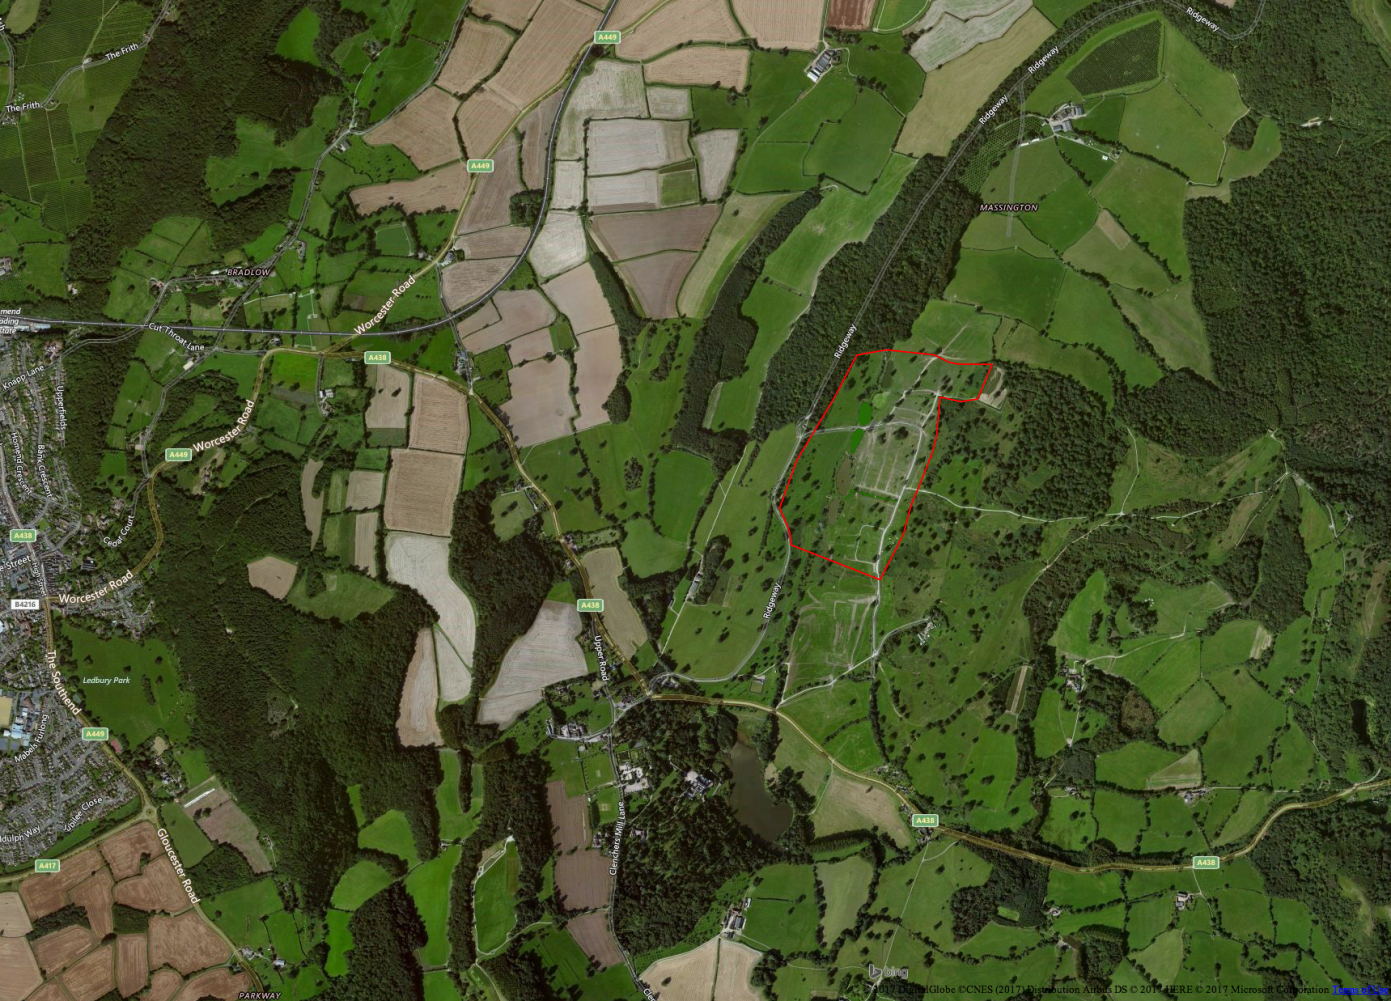
\includegraphics[width=24cm]{./supplementary/wide-map.png}
\end{landscape}
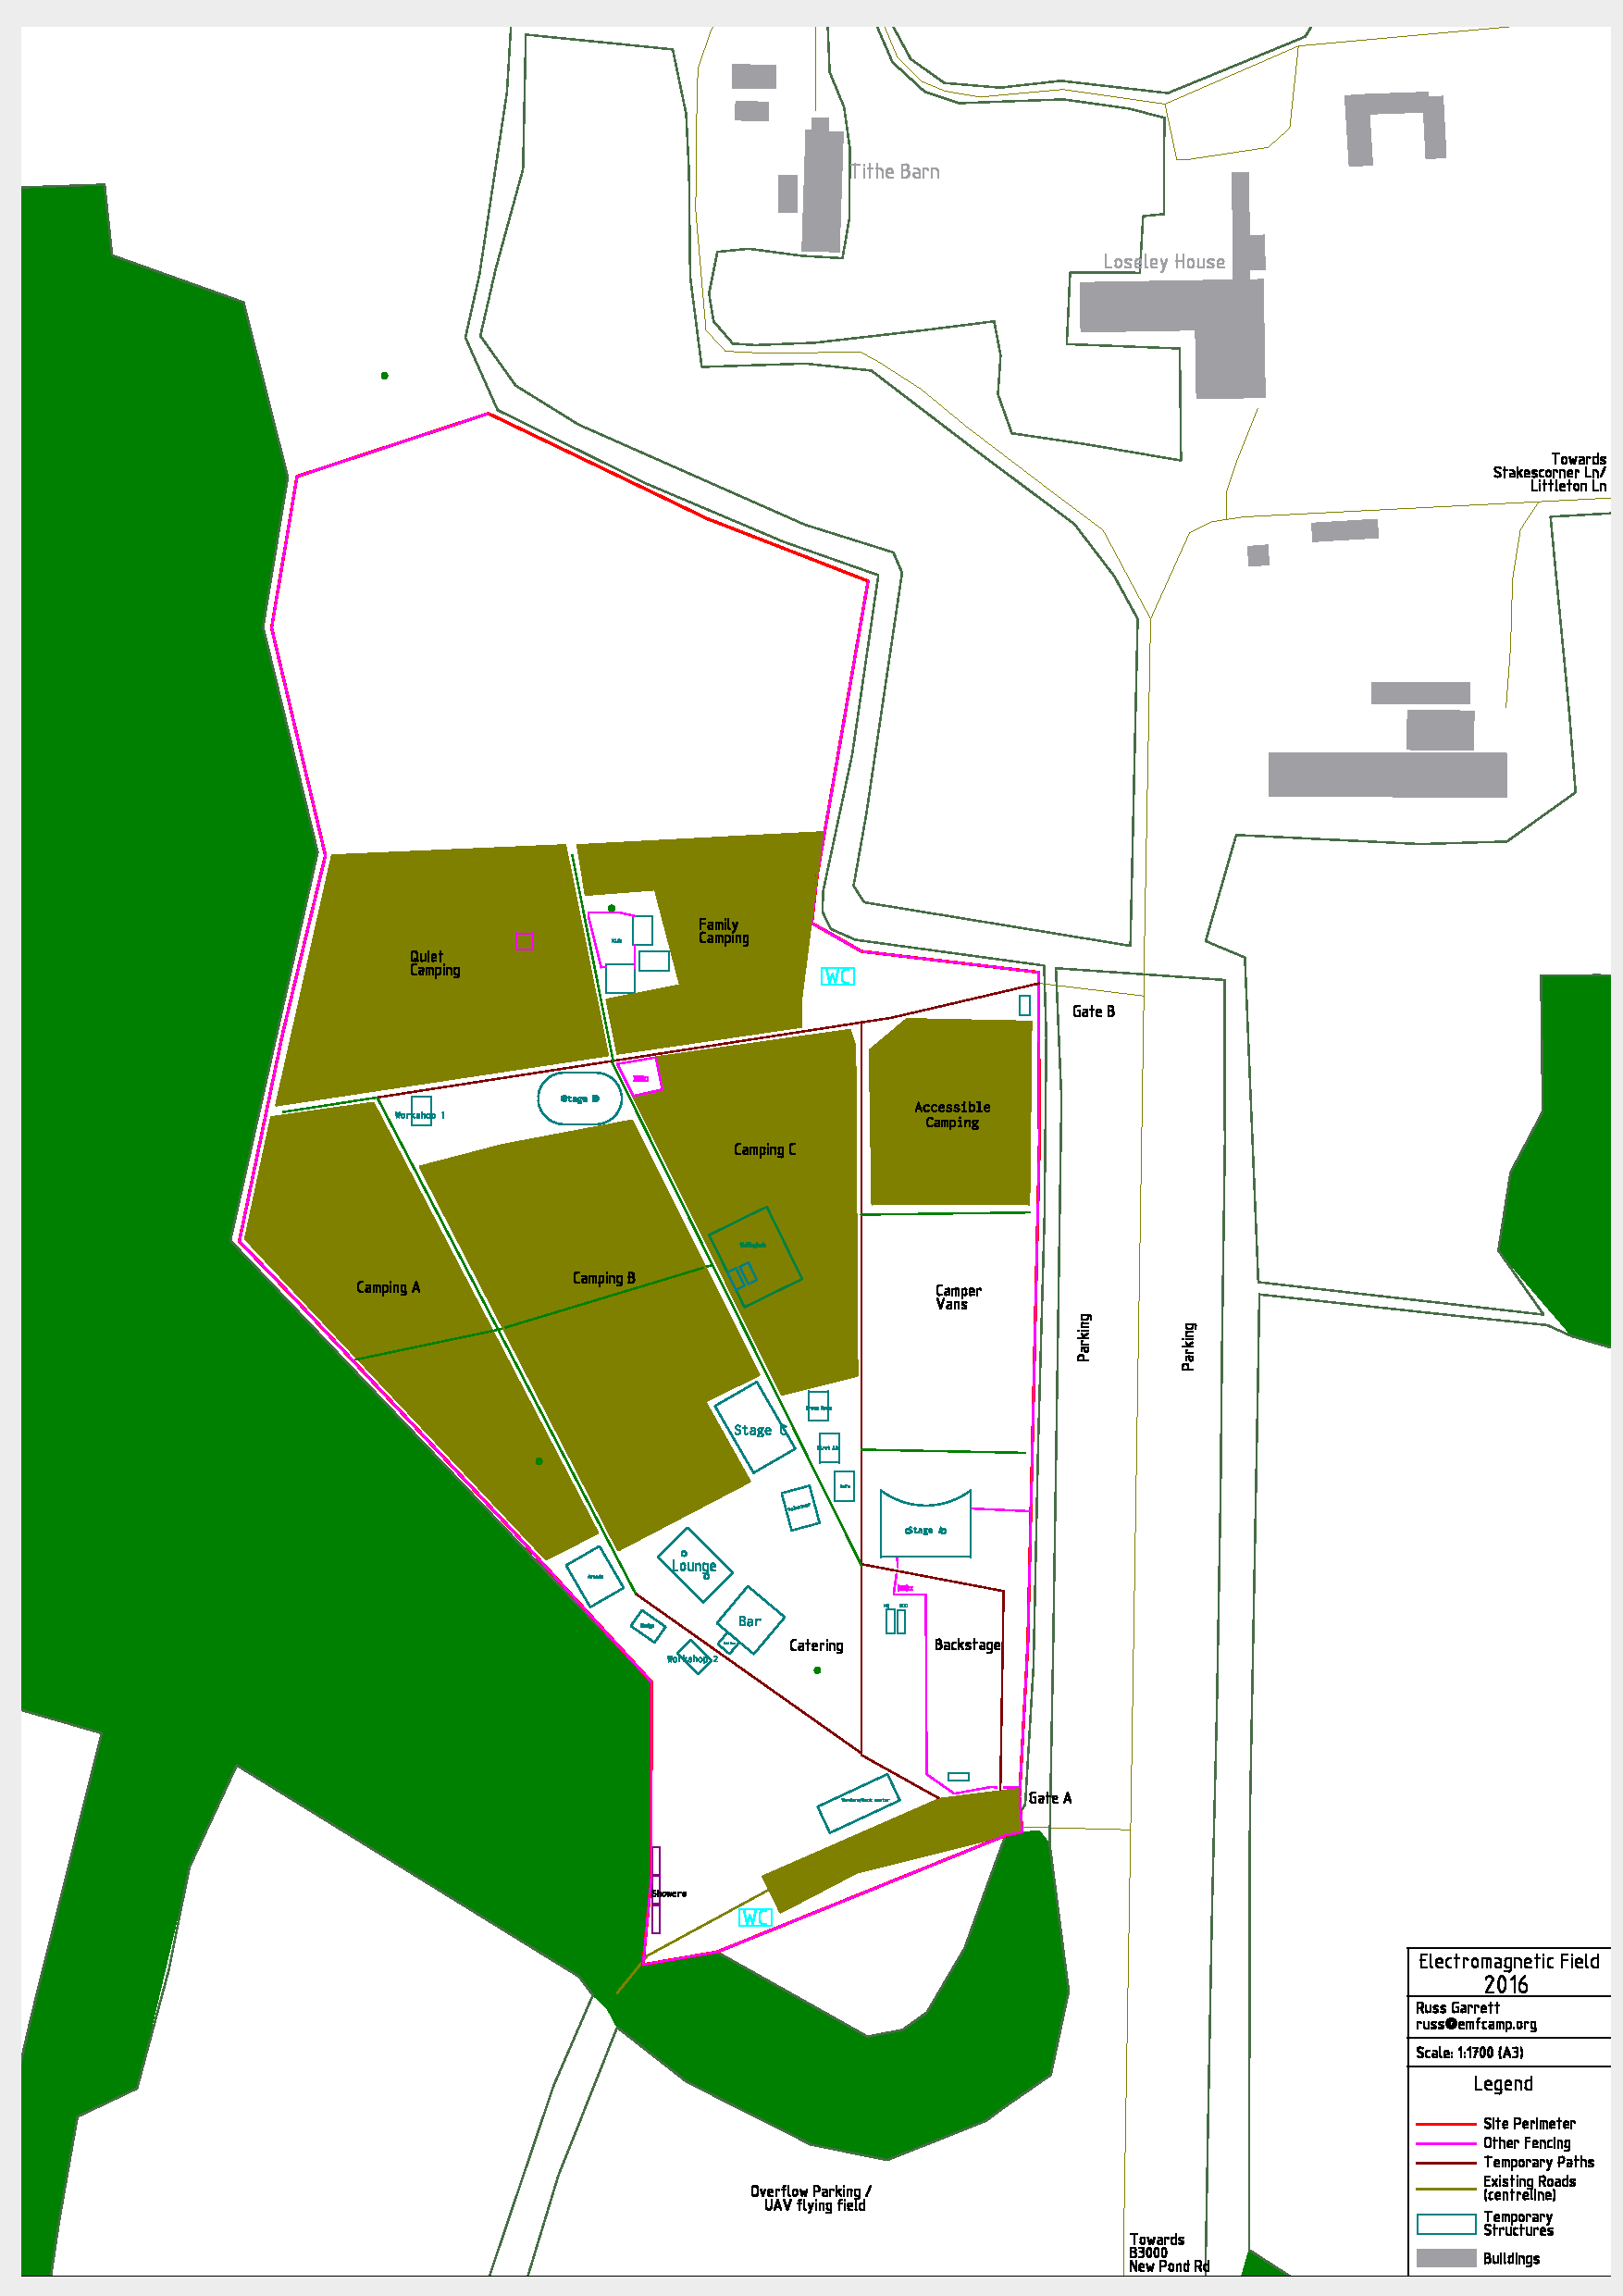
\includepdf[pages=1,fitpaper=true]{./supplementary/site-plan.pdf}

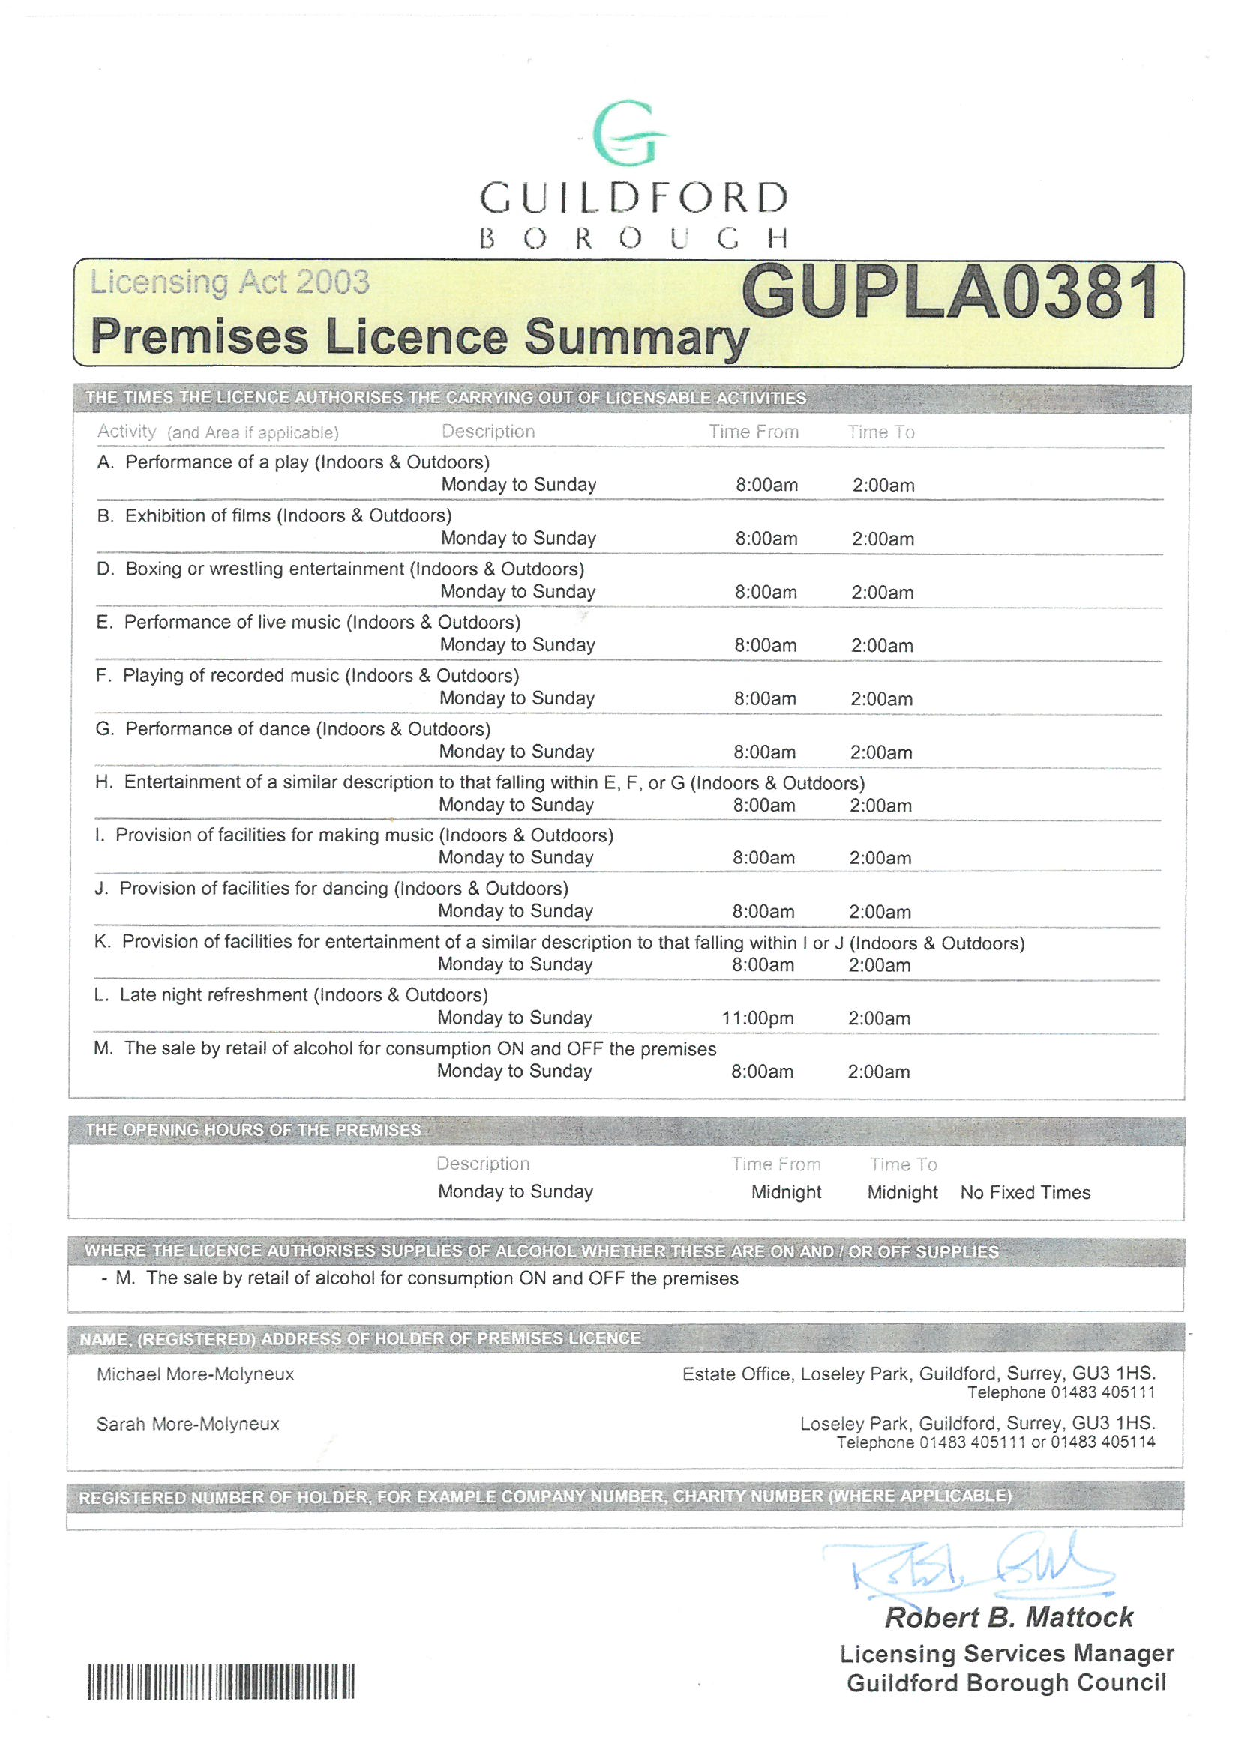
\includepdf[pages=1,scale=0.9,pagecommand=\section{Premises License}\label{premises-license}]{./supplementary/premises-license.pdf}
\includepdf[pages=2-,scale=0.9,pagecommand={}]{./supplementary/premises-license.pdf}
